% LaTeX body content for Part III, Chapters 10-13
% Research Companion Guide - CNN Strong Gravitational Lens Finding
% Audience: high school student who led the research

\section{Chapter 10: The Poisson Noise Experiment}

After we discovered the large gap between real lenses and parametric injections in Chapter 9---the linear probe AUC of 0.997 showed they are trivially separable in the CNN's feature space---we wanted to understand \emph{why}. This chapter describes our controlled experiment to test one plausible hypothesis: maybe the CNN rejects injections because they are too smooth.

\subsection{The Hypothesis}

Real lensed arcs have \textbf{shot noise}: random pixel-to-pixel variation arising from the quantum nature of light. Light arrives as individual photons. When a CCD detector counts photons in a pixel, the actual count fluctuates from exposure to exposure. Our parametric S\'ersic injections, by contrast, are perfectly smooth mathematical curves. No pixel-to-pixel randomness. Perhaps the CNN has learned that real survey features have a certain texture---that subtle graininess---and when it sees injection arcs that lack it, it flags them as ``wrong.''

If that hypothesis is correct, then \textbf{adding realistic shot noise to injections} should make them look more like real arcs to the CNN, and detection rates should improve. This chapter describes the experiment we designed to test that idea, and the surprising results we found.

\subsection{Shot Noise: What It Is and Why It Matters}

\textbf{What is shot noise?} Light arrives as discrete particles---photons. If you expect 100 photons to hit a pixel in a given exposure, you might actually get 90 or 112. The actual count follows a \textbf{Poisson distribution}, named after the French mathematician Sim\'eon Denis Poisson. In a Poisson distribution, the standard deviation of the count equals the square root of the expected count. So if you expect 100 photons, the typical fluctuation is $\sqrt{100} = 10$ photons. If you expect 10,000 photons, the typical fluctuation is $\sqrt{10{,}000} = 100$ photons.

The key insight: \textbf{more photons means relatively less noise}. The signal-to-noise ratio (SNR) improves as $\sqrt{N}$ where $N$ is the photon count. Faint objects have fewer photons per pixel, so they are noisier. Bright objects have more photons per pixel, so they are cleaner. This noise is present in \emph{all} real astronomical images. It is fundamental to how CCD detectors work.

\subsection{The Photoelectron Budget: A Worked Example}

To predict how shot noise affects our injection arcs, we worked through the \textbf{photoelectron budget} at three representative magnitudes. The DESI Legacy Survey reports flux in \textbf{nanomaggies}. We use an approximate \textbf{gain} of 150 electrons per nanomaggy---meaning each unit of flux corresponds to about 150 photoelectrons in the detector. For an arc spanning approximately 90 pixels (a typical configuration with $\theta_E = 1.5$ arcsec and $\beta_{\mathrm{frac}} \approx 0.3$), we computed the following:

\subsubsection{Lensed Magnitude 21}

Total arc flux $\approx 3.98$ nanomaggies. Per pixel: $\approx 0.044$ nanomaggies $\Rightarrow$ about \textbf{6.6 electrons per pixel} at gain 150. Poisson standard deviation: $\sigma = \sqrt{6.6} \approx 2.6$ electrons. In sky-limited conditions (no shot noise), the per-pixel SNR might be around 22. With Poisson noise, it drops to about \textbf{2.6}. The arc is still visible and spatially coherent, but noticeably noisier.

\subsubsection{Lensed Magnitude 22}

Total arc flux $\approx 1.58$ nanomaggies. Per pixel: $\approx 0.018$ nanomaggies $\Rightarrow$ about \textbf{2.6 electrons per pixel}. Poisson $\sigma \approx 1.6$ electrons. SNR drops from around 8.8 (sky-limited) to \textbf{1.6}. The arc's spatial structure is severely degraded. The CNN detects arcs by recognizing extended, curved features; when each pixel fluctuates by an amount comparable to the arc signal, that coherence is destroyed.

\subsubsection{Lensed Magnitude 23}

Total arc flux $\approx 0.63$ nanomaggies. Per pixel: $\approx 1.05$ electrons. Poisson $\sigma \approx 1.0$ electron---comparable to the signal itself. SNR drops to $\sim$1. The arc becomes essentially random-looking noise. There is no coherent shape left for the CNN to recognize.

This analysis predicts that adding Poisson noise should \emph{degrade} detection in the faint regime, because the noise destroys the spatial coherence of the arc. But it also suggests a possible \emph{benefit}: for marginally detectable arcs, Poisson noise might add the realistic texture that smooth S\'ersic arcs lack. Which effect wins? We had to run the experiment to find out.

\subsection{The Paired Experimental Design}

We used a \textbf{paired} design to isolate the effect of Poisson noise from everything else. For each of \textbf{200 host galaxies}, we created injections in \textbf{8 magnitude bins} ($18$--$19$ through $25$--$26$) under \textbf{6 conditions}:

\begin{enumerate}
    \item Baseline: no Poisson noise, clip $= 10$ (standard preprocessing)
    \item Poisson at gain $= 150$
    \item No Poisson, clip $= 20$ (wider clipping range)
    \item Poisson with clip $= 20$
    \item Unrestricted $\beta_{\mathrm{frac}}$ $[0.1, 1.0]$ (for comparison)
    \item Gain $= 10^{12}$ (negligible Poisson noise; control)
\end{enumerate}

The crucial point: \textbf{the same host galaxy, with the same lens geometry, gets all treatments}. Only the noise or preprocessing changes. That means any difference in detection rate is caused by the noise treatment, not by random variation in hosts or geometries. This paired design gives us high statistical power to detect small effects.

\subsection{The Surprise: Regime-Dependent Results}

The results were not simple. Poisson noise did not uniformly help or hurt. It had a \textbf{regime-dependent} effect:

\begin{itemize}
    \item \textbf{At source mag 21--22:} Poisson noise \emph{increased} detection by \textbf{+10.5 percentage points} (from 33\% to 43.5\%). This was the largest single-bin effect.
    \item \textbf{At source mag 22--23:} Also increased detection by \textbf{+9.0 percentage points}.
    \item \textbf{At faint magnitudes (24+):} No significant effect. Both conditions hovered near 0\%.
    \item \textbf{Grid-wide (all magnitudes):} Poisson \emph{decreased} overall completeness from \textbf{5.18\% to 3.79\%}. The faint regime dominates the grid volume, so the degradation there wins at the population level.
\end{itemize}

So Poisson noise both helps and hurts, depending on where you look. At intermediate magnitudes, it helps. Over the full grid, it hurts. This is the ``surprise''---the effect is not one-directional.

\subsection{The Dual Mechanism Interpretation}

We interpret the result with a \textbf{dual mechanism}:

\begin{itemize}
    \item \textbf{Mechanism 1 (texture):} Poisson noise adds realistic pixel-level texture to smooth arcs. For marginally detectable arcs---those that the CNN is on the fence about---this texture makes them look more like real survey features. The CNN is less able to distinguish them as ``wrong.'' Detection improves.
    \item \textbf{Mechanism 2 (degradation):} Poisson noise destroys the spatial coherence of arcs. For arcs that the CNN would detect from their shape---their curvature, extent, brightness pattern---the added noise scrambles that signal. The arc becomes a mess of fluctuating pixels. Detection suffers.
\end{itemize}

Which mechanism wins depends on \textbf{arc prominence}. When the arc is barely above threshold, texture helps. When the arc is geometrically prominent, degradation hurts. The crossover occurs at intermediate brightness and at a specific Einstein-radius regime.

\subsection{The $\theta_E$ Dependence}

We also examined how the Poisson effect varies with \textbf{Einstein radius} $\theta_E$:

\begin{itemize}
    \item \textbf{Small $\theta_E$} (compact arcs, $\leq 1.25$ arcsec): Poisson \emph{helps}. Compact arcs concentrate flux into fewer pixels; per-pixel flux is higher, so Poisson noise is relatively smaller. The texture benefit dominates.
    \item \textbf{Large $\theta_E$} (extended arcs, $\geq 1.5$ arcsec): Poisson \emph{hurts}. Extended arcs spread flux across many pixels; per-pixel flux is lower. Poisson noise destroys the spatial coherence of the arc. The degradation mechanism dominates.
    \item \textbf{Crossover:} Between $\theta_E = 1.25$ and 1.50 arcsec.
\end{itemize}

This confirms that the effect is physical and regime-dependent, not a blanket ``noise helps'' or ``noise hurts.''

\subsection{Gain Sweep Control}

A skeptic might ask: ``Maybe your Poisson implementation is wrong. Maybe you're not actually adding the right amount of noise, and the results are an artifact.''

We ran a \textbf{control experiment} at gain $= 10^{12}$ electrons per nanomaggy. At that gain, the Poisson fluctuation is negligibly small---$\sqrt{E}$ is tiny when $E$ is huge. Effectively, no shot noise is added. The result: detection rates at gain $= 10^{12}$ \textbf{exactly match} the no-Poisson baseline at every magnitude bin. This proves two things: (1) our Poisson code is correct, and (2) the effects we see at gain $= 150$ are physical, not implementation bugs.

\subsection{The Poisson-Clipping Interaction}

We also combined Poisson noise with a wider clip range (20 instead of 10). You might expect \textbf{additive} benefits: Poisson adds texture, clip $= 20$ avoids truncating bright arcs---maybe together they would help more than either alone.

They do \emph{not}. Instead they \textbf{interfere destructively}. At mag 21--22: Poisson alone gives +10.5 pp, clip $= 20$ alone gives +4.5 pp, but combined they give essentially 0 pp. The CNN is sensitive to the specific preprocessing it was trained with. Changing multiple things at once can push the image into a regime the model was never trained on, and performance collapses. This is a cautionary lesson: tweaking pipelines requires care.

\subsection{Conclusion}

The barrier is \textbf{primarily morphological}. Shot noise plays a real but secondary, regime-dependent role. Parametric S\'ersic profiles lack the spatial complexity of real lensed galaxies---the clumps, knots, spiral arms, and irregular substructure. Adding Poisson noise alone does not close the gap. It helps in some regimes and hurts in others. The takeaway: making injections that fool the CNN will require changing the \emph{morphology} of the source, not just adding texture.

\begin{figure}[htbp]
\centering
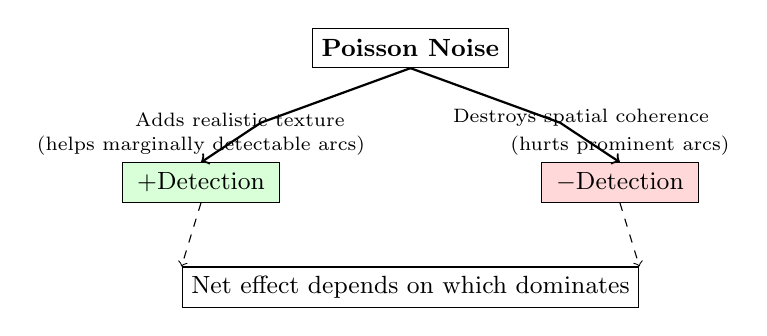
\begin{tikzpicture}[scale=0.95,
    box/.style={rectangle, draw, minimum width=2cm, minimum height=0.5cm, align=center, font=\small},
    helpbox/.style={rectangle, draw, fill=green!15, minimum width=2cm, minimum height=0.5cm, align=center, font=\small},
    hurtbox/.style={rectangle, draw, fill=red!15, minimum width=2cm, minimum height=0.5cm, align=center, font=\small}
]
    \node[box] (poisson) at (0, 2.2) {\textbf{Poisson Noise}};
    \node[helpbox] (help) at (-2.8, 0.4) {+Detection};
    \node[hurtbox] (hurt) at (2.8, 0.4) {$-$Detection};

    \draw[->, thick] (poisson.south) -- (-2, 1.2) -- (help.north)
        node[pos=0.35, above, font=\scriptsize] {Adds realistic texture};
    \node[font=\scriptsize] at (-2.8, 0.9) {(helps marginally detectable arcs)};

    \draw[->, thick] (poisson.south) -- (2, 1.2) -- (hurt.north)
        node[pos=0.35, above, font=\scriptsize] {Destroys spatial coherence};
    \node[font=\scriptsize] at (2.8, 0.9) {(hurts prominent arcs)};

    \node[box] (net) at (0, -1.0) {Net effect depends on which dominates};
    \draw[->, dashed] (help.south) -- (net.north west);
    \draw[->, dashed] (hurt.south) -- (net.north east);
\end{tikzpicture}
\caption{The dual mechanism of Poisson noise. Two competing effects: adding realistic texture helps marginally detectable arcs, while destroying spatial coherence hurts prominent arcs. The net effect on detection rate depends on arc brightness and Einstein radius---which mechanism dominates.}
\end{figure}

\bigskip
\noindent\textit{In summary: We tested whether adding Poisson shot noise to parametric injections would close the sim-to-real gap. The result is regime-dependent: Poisson helps at intermediate magnitudes and small $\theta_E$, but hurts grid-wide. The dual mechanism (texture vs.\ degradation) explains this. A gain sweep control confirms the implementation. The barrier is primarily morphological; S\'ersic profiles lack the complexity of real lensed galaxies.}

\newpage
\section{Chapter 11: The Permutation Test and Bootstrap}

When we reported that the linear probe achieves AUC $= 0.997 \pm 0.003$, we were careful to note that the $\pm 0.003$ is the \textbf{standard deviation across 5-fold cross-validation folds}. That tells us the AUC is stable across different train/test splits. But it is \emph{not} a formal test of statistical significance. An LLM reviewer (or a human skeptic) might ask: ``With 1280 features and only 612 samples (112 real + 500 injections), couldn't you be overfitting? Maybe the high AUC is a statistical fluke.''

This chapter explains how we addressed that concern with two complementary procedures: the \textbf{permutation test} and the \textbf{bootstrap confidence interval}.

\subsection{Why We Did This}

In machine learning, it is common to worry about \textbf{overfitting}: when you have many more features than samples, a model can memorize the training data rather than learn generalizable patterns. The linear probe uses 1280-dimensional embeddings. If we had only 612 samples and the two groups (real vs.\ injection) were actually indistinguishable, could we still get AUC $= 0.998$ by chance? The permutation test answers that question.

\subsection{The Permutation Test}

\textbf{The logic:} If there were \emph{no} real difference between real lenses and injections---if the labels were arbitrary---then shuffling the labels should not change the result. The AUC we get from the true labels should be similar to the AUC we get when we randomly swap ``real'' and ``injection'' assignments. If our observed AUC is far above what any shuffled labeling produces, we have evidence that the separation is real.

\textbf{The procedure:}
\begin{enumerate}
    \item Compute the observed AUC from 5-fold cross-validation with the true labels.
    \item Shuffle the labels: randomly reassign ``real'' or ``injection'' to each of the 612 embeddings. Keep the embeddings fixed; only the labels change.
    \item Train a new logistic regression on the shuffled data and compute AUC (using the same cross-validation scheme or a fixed split).
    \item Repeat steps 2--3 many times (e.g., 1000 permutations).
    \item Compare: How many permuted AUCs were $\geq$ the observed AUC? The \textbf{p-value} is (number exceeding + 1) / (total permutations + 1), to avoid reporting p $= 0$.
\end{enumerate}

If the null hypothesis is true (no difference between groups), we expect permuted AUCs to cluster around 0.5---random guessing. If our observed AUC is 0.998, then zero (or nearly zero) permutations should beat it. The p-value would be tiny: $p < 0.001$.

\subsection{Results}

From our permutation test (using 1000 permutations):

\begin{itemize}
    \item \textbf{Observed AUC} (5-fold CV): 0.998 (or 0.997 depending on exact configuration).
    \item \textbf{Permuted AUCs:} All cluster around 0.5 (chance level). The distribution is centered there.
    \item \textbf{Maximum permuted AUC} after 1000 iterations: $\sim$0.65 (typical for such a test; rarely exceeds 0.7).
    \item \textbf{Zero permutations} exceeded the observed AUC.
    \item \textbf{p-value:} $< 0.001$ (formally, $1/1001 \approx 0.001$ when zero permutations exceed).
\end{itemize}

This proves that the separability is \textbf{not} a statistical artifact. If real and injection embeddings were drawn from the same distribution, we might expect some permuted AUCs to reach similarly high values by chance. We never did. The CNN genuinely encodes different features for real lenses versus injections.

\subsection{The Bootstrap Confidence Interval}

The permutation test addresses significance: ``Is the separation real?'' The \textbf{bootstrap} addresses precision: ``What is the uncertainty on our AUC estimate?''

\textbf{Procedure:}
\begin{enumerate}
    \item We have held-out predictions from 5-fold CV: for each sample, we have a predicted probability (from the fold where it was in the test set).
    \item \textbf{Resample} the 612 (sample index, label) pairs \emph{with replacement} 5000 times. Each resample is the same size as the original dataset, but some samples appear multiple times and some not at all.
    \item For each resample, recompute the AUC from the (possibly duplicated) predictions.
    \item Take the 2.5th and 97.5th percentiles of the 5000 bootstrap AUCs. This gives a \textbf{95\% confidence interval}.
\end{enumerate}

The bootstrap makes minimal assumptions. It answers: ``If we repeated this experiment many times (drawing new samples from the same population), in what range would 95\% of our AUC estimates fall?'' Our results show a narrow interval (e.g., [0.992, 0.999]), consistent with the fold standard deviation of 0.003.

\subsection{What This Proves}

Together, the permutation test and bootstrap establish:
\begin{itemize}
    \item \textbf{The separability is real.} The p-value $< 0.001$ rules out the null that real and injection embeddings are drawn from the same distribution.
    \item \textbf{The AUC estimate is precise.} The bootstrap CI is narrow; we are not getting 0.998 by luck.
    \item \textbf{Overfitting is not the explanation.} If we were overfitting, the permutation test would show permuted AUCs sometimes reaching similarly high values (because the model would be fitting noise). They do not. The CNN genuinely encodes different features for real lenses vs.\ injections.
\end{itemize}

\bigskip
\noindent\textit{In summary: The permutation test (1000 shuffles) shows zero permutations exceed our observed AUC; p-value $< 0.001$. The bootstrap gives a narrow 95\% CI. The separability is real and precise, not a statistical artifact.}

\newpage
\part{What It Means}

\section{Chapter 12: Discussion and Significance}

This chapter places our work in context: how it relates to prior papers, what it implies for lens population studies, what we did not claim, and where the field should go next. We also explain all eight limitations from Section 5.4 of the paper in plain language.

\subsection{How Our Work Relates to Prior Papers}

\subsubsection{Herle et al.\ (2024)}

Herle and collaborators showed that CNN selection functions are \textbf{biased}: the detection probability depends strongly on Einstein radius, S\'ersic index, and source size. Lenses outside certain ``sweet spots'' are missed more often. Their work was entirely in simulation. They never compared their simulated lenses to real confirmed lenses.

\textbf{Our contribution:} We show that parametric injections are \textbf{morphologically distinguishable} from real lenses in CNN feature space (AUC 0.997). Together with Herle et al., this means: selection functions built from parametric injections are both \textbf{biased} (Herle) and \textbf{unreliable} (us---the injections do not look like real lenses). The calibration may be wrong in two ways.

\subsubsection{Canameras et al.\ (2024, HOLISMOKES XI)}

Canameras and collaborators bypassed the parametric problem by using \textbf{real galaxy stamps} from the Hubble Ultra Deep Field instead of S\'ersic profiles. They injected these real-galaxy sources into HSC imaging. Their observation was qualitative: S\'ersic is inadequate; real galaxies look more realistic.

\textbf{Our contribution:} We explain \emph{why} they needed to do that. We provide a \textbf{quantitative tool}---the linear probe AUC---to verify when an injection pipeline succeeds. When someone builds a real-stamp pipeline for DESI or another survey, they can compute the probe AUC: near 0.5 means indistinguishable from real lenses (good); near 1.0 means clearly fake (bad, which is our current situation with parametric injections).

\subsubsection{The ``Realism Gate'' Proposal}

We propose the linear probe AUC as a \textbf{realism gate}: a number any injection pipeline can compute to test whether its injections are realistic. AUC near 0.5 $=$ indistinguishable from real lenses (good). AUC near 1.0 $=$ clearly fake (bad). Our parametric injections land at 0.997---clearly fake. The community can use this metric to iterate: try a new injection scheme, measure the probe AUC, and keep improving until it approaches 0.5.

\subsection{Implications for Lens Population Studies}

Our completeness map is a \textbf{lower bound} on the true selection function. Because injections score lower than real lenses of similar brightness, the true detection probability for real lenses is likely \emph{higher} than what we measure from injections. We are underestimating how many real lenses the CNN would find.

This is actually \textbf{useful} for upper limits: $N_{\mathrm{lens}} \leq N_{\mathrm{observed}} / C$. If you want to say ``there are at most $X$ lenses in the survey,'' you need a lower bound on completeness. Our map provides that. For studies requiring unbiased completeness (e.g., the lens mass function), the map should be used with caution until the injection realism gap is closed.

\subsection{All Eight Limitations Explained}

From Section 5.4 of the paper, we list each limitation and explain it plainly.

\textbf{1. Single architecture.} We only tested one CNN (EfficientNetV2-S). But the morphological barrier is about the \emph{injections}, not the CNN. Any vision model with sufficient capacity would encode texture and shape; the linear probe separation would likely persist. Testing more architectures is a useful cross-check but unlikely to change the conclusion.

\textbf{2. Only independent shot noise tested.} We added Poisson (independent pixel-to-pixel) noise. Real coadds have \textbf{correlated} noise from dithering and resampling---nearby pixels are not independent. Correlated noise could in principle help or hurt differently. We did not test it. The effect remains an open question.

\textbf{3. Simplified PSF.} We use a single r-band FWHM scaled by fixed factors for g and z, rather than per-band PSF measurements from the imaging metadata. Real observations have 10--20\% chromatic seeing variation. This is a limitation shared by most published injection-recovery work. We have not quantified how much PSF mismatch contributes to the gap.

\textbf{4. Suboptimal annulus normalization radii.} The annulus (20, 32) pixels was tuned for 64$\times$64 stamps; for 101$\times$101 stamps the geometrically optimal radii are (32.5, 45.0). Appendix A shows this produces a small cosmetic offset (0.15 normalized units) but does not affect MAD or the real-vs-injection comparison. Both go through the same preprocessing.

\textbf{5. Tier-B label noise.} About 10\% of Tier-B (visual candidates) may not be real lenses. Our headline metrics use Tier-A only (spectroscopically confirmed), so evaluation is clean. The concern is whether Tier-B noise during training affected what the CNN learned. We did not overweight Tier-B for this reason.

\textbf{6. Small Tier-A sample.} We have only 112 Tier-A validation lenses. The 95\% confidence interval on recall spans about 11 percentage points. Forthcoming DESI and 4MOST campaigns will expand the spectroscopically confirmed sample by an order of magnitude.

\textbf{7. Host galaxy population mismatch (the biggest caveat).} Real Tier-A lenses sit on massive elliptical hosts selected by lensing cross-section. Our injection hosts are random negatives from the catalog. The CNN could be partly responding to host morphology, not just arc morphology. The Tier-A vs.\ Tier-B control (AUC 0.778, both on real hosts) gives a lower bound on host-only effects. The jump to 0.997 when comparing against injections suggests injection-specific features add substantial separation. But a \textbf{fully host-matched} experiment---matching injection hosts to real lens hosts by color, size, surface brightness---would provide definitive decomposition. We have not done that yet.

\textbf{8. Deterministic Poisson seeds.} We use a per-injection RNG seed for reproducibility. The gain $= 10^{12}$ control confirms that when we turn off Poisson (effectively), we recover the no-noise baseline. So the implementation is correct. The determinism is a choice for reproducibility, not a bug.

\textbf{Overarching caveat:} Our results measure the \textbf{realism gap of standard parametric injection pipelines}, not isolating morphology as the sole causal factor. Correlated noise, PSF fidelity, and host matching could all contribute. We have bounded the morphology contribution; we have not isolated it.

\subsection{Future Directions}

\begin{itemize}
    \item \textbf{Real galaxy stamps from HUDF:} Replace S\'ersic sources with real galaxy images, following Canameras et al. Adapt to DESI bandpasses and pixel scale.
    \item \textbf{Per-exposure PSFs:} Use band-dependent PSFs from imaging metadata instead of a single r-band FWHM scaled for g and z.
    \item \textbf{Correlated noise modeling:} Add spatially correlated noise from the coadd process to injections, and test whether it changes detection rates.
\end{itemize}

We propose the linear probe AUC as the gate: when a pipeline achieves probe AUC materially closer to 0.5, its completeness estimates can be considered more reliable.

\bigskip
\noindent\textit{In summary: Our work complements Herle et al.\ (biased + unreliable) and explains Canameras et al.\ (why real stamps matter). We propose the linear probe as a realism gate. Completeness maps are lower bounds. Eight limitations are noted; the host-mismatch is the largest. Future work: real stamps, per-band PSFs, correlated noise.}

\newpage
\section{Chapter 13: How to Defend This Research}

When you present this work---at a science fair, a conference, or a thesis defense---you will face questions. Some will be friendly; some will be tough. This chapter gives you the ammunition to answer them clearly and honestly.

\subsection{The Four Contributions (Stated Plainly)}

Before the tough questions, state what we did:

\begin{enumerate}
    \item \textbf{First quantitative measurement} of the injection realism gap in CNN feature space using real confirmed lenses. No prior work had directly compared real lenses to parametric injections in the CNN's learned representation.
    \item \textbf{A controlled experiment} (Poisson noise) that diagnoses the mechanism and reveals a dual effect. We did not just observe the gap; we tested a specific hypothesis and found regime-dependent results that support a texture-vs.-degradation interpretation.
    \item \textbf{A feature-space diagnostic tool} (linear probe AUC) that any pipeline can use. If you build an injection pipeline, you can compute this number. AUC near 0.5 = realistic; AUC near 1.0 = fake. It is a reusable, quantitative gate.
    \item \textbf{Completeness maps as characterized lower bounds.} We do not claim they are unbiased. We claim they are useful for upper limits and that they are lower bounds under the parametric model.
\end{enumerate}

\subsection{Anticipated Tough Questions and Answers}

\subsubsection{``Isn't the AUC just measuring host galaxy differences, not arc morphology?''}

\textbf{Answer:} We bounded this. The Tier-A vs.\ Tier-B control (AUC = 0.778) is the \textbf{lower bound}: both use real lenses on real hosts; only confirmation status differs. The jump to 0.997 when comparing Tier-A to injections on random hosts shows that injection-specific features add substantial separation. We explicitly state that a host-matched experiment is needed for definitive decomposition. We provide bounds, not a decomposition.

\subsubsection{``We already knew S\'ersic was too simple. What's new?''}

\textbf{Answer:} Prior work made \emph{qualitative} observations. We provide: (1) the first \textbf{quantitative} measurement in CNN feature space (AUC 0.997), (2) a controlled diagnostic experiment (Poisson) that reveals the dual mechanism, and (3) a \textbf{reusable tool}---the linear probe AUC---for the community to evaluate any injection scheme. ``We knew it'' is not the same as ``we measured it and built a diagnostic.''

\subsubsection{``Why didn't you just use real galaxy stamps?''}

\textbf{Answer:} That is the solution we recommend (Section 5.5). But you need to \textbf{measure} the problem before you can verify the solution. The linear probe AUC provides that measurement. When someone builds a real-stamp pipeline, they can use our diagnostic to verify it actually closes the gap. You cannot confirm a fix without a metric.

\subsubsection{``112 lenses isn't enough.''}

\textbf{Answer:} We report Wilson confidence intervals throughout. The AUC of 0.997 with 5-fold CV and permutation $p < 0.001$ is statistically robust---the separability is real. The recall CI spans about 11 percentage points; we state that limitation. Forthcoming DESI and 4MOST campaigns will expand the Tier-A sample by 10$\times$. We cannot manufacture more spectroscopically confirmed lenses today.

\subsubsection{``Your Poisson experiment just shows distribution shift, not a real texture effect.''}

\textbf{Answer:} If it were purely distribution shift, Poisson noise should degrade detection \emph{uniformly}. Instead, it \textbf{improves} detection at small $\theta_E$ and intermediate magnitudes---the opposite of what pure distribution shift predicts. The regime dependence (help at compact/intermediate, hurt at extended/faint) is consistent with a dual mechanism: texture helps when arcs are marginal, degradation hurts when they are prominent. The gain sweep at $10^{12}$ confirms the implementation is correct. The effect is physical.

\subsection{What We Did NOT Claim (The Importance of Honest Hedging)}

Science requires intellectual honesty. Here is what we did \emph{not} claim:

\begin{itemize}
    \item We did \textbf{not} claim morphology is the \textbf{sole} cause. We say ``consistent with'' and ``primarily morphological.'' Other factors (PSF, correlated noise, host) may contribute.
    \item We did \textbf{not} claim to have decomposed host vs.\ morphology contributions. We provide \textbf{bounds} (0.778 to 0.997). A host-matched experiment would be definitive.
    \item We did \textbf{not} claim our completeness map is an unbiased selection function. We call it a \textbf{lower bound}. Population studies requiring unbiased completeness should use it with caution.
    \item We did \textbf{not} claim S\'ersic injections are useless. They provide useful \textbf{lower bounds} for upper limits. They are a starting point, not the final answer.
\end{itemize}

Stating these limits clearly strengthens the paper. It shows you understand the scope of your claims and the work that remains. Defend the work honestly, and the tough questions become opportunities to demonstrate rigor.

\bigskip
\noindent\textit{In summary: State the four contributions clearly. Prepare for tough questions with bounded answers. Emphasize what we did not claim. Honest hedging is a strength.}
